\documentclass[tikz]{standalone}
\usetikzlibrary{calc}
\usepackage{pgfplots}
\usepgfplotslibrary{polar}
\pgfplotsset{compat=1.13}

\begin{document}

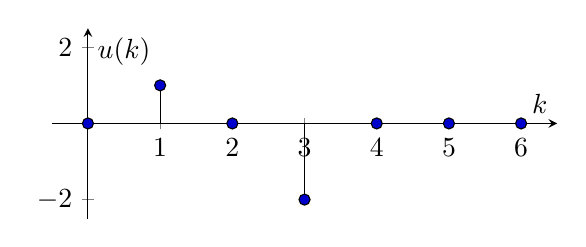
\begin{tikzpicture}
\begin{axis}[
  width=8cm,
  height=4cm,
  xlabel={$k$},
  ylabel={$u(k)$},
  axis lines=middle,
  xmin=-.5,
  xmax=6.5,
  ymin = -2.5, ymax = 2.5,
  xtick = {1,2,3,4,5,6},
]

\addplot+[black, ycomb, domain=-2:10, samples=13,variable=k] { (k==1) - 2*(k==3)}; 

\end{axis}
\end{tikzpicture}
\end{document}
